\documentclass{beamer}

\mode<presentation>
{
\usetheme{Warsaw}

\setbeamercovered{transparent}
}

\usepackage[english]{babel}
\usepackage[latin1]{inputenc}
\usepackage{amsfonts}
\usepackage{amsmath}
\usepackage{mathtools}

\usepackage[scaled=.90]{helvet}
\usepackage{courier}
\usepackage{graphicx}
\usepackage{color}
\usepackage{subfig}
\DeclareGraphicsExtensions{.pdf,.png,.jpg,.mps}
\usepackage[absolute,overlay]{textpos}
\setlength{\TPHorizModule}{1mm}
\setlength{\TPVertModule}{1mm}
\usepackage{ragged2e}
\justifying
\usepackage{color}
\usepackage{physics}
\usepackage{mathtools}
\usepackage{amsmath}
\usepackage{bm}
\usepackage{calc}
\usepackage{listings}
\usepackage{url}
\usepackage{rotating}
%\usepackage{calrsfs}
\usepackage{amsfonts}
\usepackage[T1]{fontenc}

%%%% A NEW COMMAND TO FIX LOGO POSITION (x,y) in mm
\newcommand{\MyLogo}{%
\begin{textblock}{13}(88,74)
%  \pgfuseimage{logo}
 
\includegraphics[height=1cm, angle=0]{images/pdp2016}
\end{textblock}
} 

\newcommand{\MyLogoo}{%
\begin{textblock}{15}(4,74)
%  \pgfuseimage{logo}
 
\includegraphics[height=1.5cm, angle=0]{images/logo1}
\end{textblock}
}
%%%% A NEW COMMAND TO FIX LOGO POSITION (x,y) in mm

%%%%%%%%%%%%%%%%%%%%%%%%%%%%%%%%%%%%%%%%%%%%%%%%%%%%%%%%%%%%%%%%%%%%%%%%%

\title[The ACIADDRI model]{Multi-Agent System with Multiple Group Modelling
for Bird Flocking on GPU}

\author{R. Hidayat\inst{1}, D. Spataro, E. De Giorgio, W. Spataro, D. D'Ambrosio\inst{2}}
\institute[shortinst]{\inst{1} BPJS Kesehatan, Indonesia \and %
	\inst{2} University of Calabria, Department of Mathematics and Computer Science}
\date{PDP 2016,  Heraklion Crete, Greece \\
February 18th, 2016}

\begin{document}

\begin{frame}
\MyLogo
\MyLogoo
\titlepage
\end{frame}

\begin{frame}{Synopsis}
\textbf{Birds flocking} is an interesting and widely studied natural phenomenon. In this paper, we present a \textbf{GPGPU model} for birds flocking simulation using NVIDIA's CUDA framework. 

Flocking simulation has important applications (to cite few) in \textit{swarm behaviour analysis} and \textit{cinema industry special effects}.

The main contributions of this paper are:
\begin{itemize}
\item improved model for multiple species aggregate motion with predator avoidance.
\item  Interactive simulation of very large number of birds
\end{itemize} 

The work shows that the use of the CUDA technology can be effective to cut computational costs also in multi-agent modelling.
\end{frame}

\begin{frame}{Contents}
\tableofcontents
\end{frame}

\section{Introduction}
\begin{frame}{Introduction}
 Flocking behaviour exists in nature at almost every length scale of observation.

A possible approach for its study is based:
\begin{itemize}
\item random motion, organisms are treated like gas molecules their motion is Brownian combined with attraction/repulsion forces;
\item differential equation (DE) models.
\end{itemize}
However organisms seldom move really randomly, nor are they just
simple particles. 
\begin{center}
$\Big{\downarrow}$ 
\end{center}

Individual-based models or even multi-agent models seem a
better choice.  
\end{frame}

\begin{frame}

ACIADDRI (\textit{Aggregate
Collection of Interactive Agents using nviDia's cuDa Reliable
Informatics}) multi-agent flocking model extends Reynolds works on bird flocking behaviour by adding 
\begin{itemize}
\item multi-species interaction
\item  predator avoidance
\item partially observable environment and birds flight constraints
\end{itemize}
We carried out experiment considering:
\begin{itemize}
\item aggregate motion of a huge number
(up to $10^7$) of boids
\item other species or predators avoidance. 
\end{itemize}
Significant performance
improvement in terms of speedup were obtained \textbf{(up to 500x)}.
\end{frame}

\section{The ACIADDRI model}
\begin{frame}{The ACIADDRI model}
Craig W. Reynolds in 1987  was among
the firsts to abstract the flocking behaviour. In his model every boid obeys to three behavioural rules:
\begin{description}
\item[COHESION: ] to attempt to stay close to nearby flockmates;
\item[COLLISION AVOIDANCE/SEPARATION: ] \hfill \\ 
to evade obstacles and flockmates which are too
close;
\item[VELOCITY/HEADING MATCHING:]\hfill \\
also called \textit{alignment}, to head in the same direction
of nearby flockmates.
\end{description}
This work extends Reynolds's model adding:
\begin{itemize}
	\item multiple group and species interaction
	\item predators avoidance
\end{itemize}
\end{frame}

\subsection{Model parameters}
\begin{frame}
\textcolor{blue}{\underline{Model parameters:}}

In ACIADDRI model the environment and each bird's
species is described by sets of parameters.

\medskip
\underline{\textbf{\textit{Environment parameters: }}}

\begin{table}[h!]
	\centering
	\begin{tabular}{ l l l l }
	\hline
	Name & Symbol & Dimension & Description\\
	\hline
	Length &  $W_x$ & $[\mathbf{L}]$ & Length of the environment \\
	Height & $W_y$ & $[\mathbf{L}]$ & Height of the environment \\
	Width & $W_z$ & $[\mathbf{L}]$ & Width of the environment \\
	Time Step & $t$ & $[\mathbf{T}]$ & Computational step duration \\
	\hline
	\end{tabular}
	\caption[List of Environment Parameters]{List of Environment Parameters of Birds Flocking}
	\label{tab:EnvironmentParameters}
\end{table}
1 pixel $\backsim$ 1 meter.

1 time step $\backsim$  1 processing time.
\end{frame}

\begin{frame}
\underline{\textbf{\textit{Species parameters: }}}

Each specie is described by a set of parameters that represent
quantities that are involved in the flight and flocking dynamics.
\begin{itemize}
\item Bird's wingspan $s$ is  an approximation of the
volume it occupies;
\item $v_p$ is the maximum velocity it can travel
and $a$ is bird's maximum acceleration.
\end{itemize}
Viewing frustum: Filed of View (FOV) together with the maximum sight distance.
\begin{center}
\begin{columns}
\column{.5\textwidth} 
\begin{figure}[h!]
		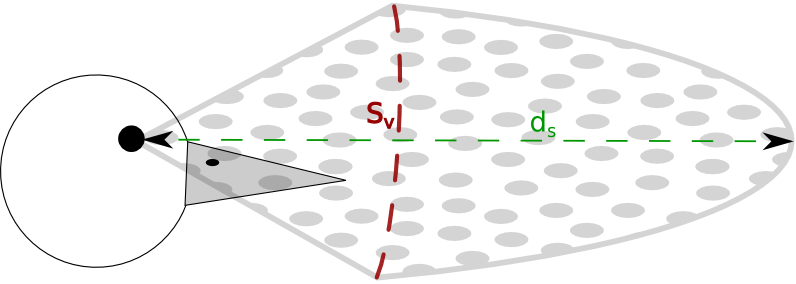
\includegraphics[scale=0.23]{images/verticalFow}
		\label{fig:vFOV}
		\caption{Birds vertical field of view. }
\end{figure}	

\column{.5\textwidth} 
\begin{figure}[h]
\centering
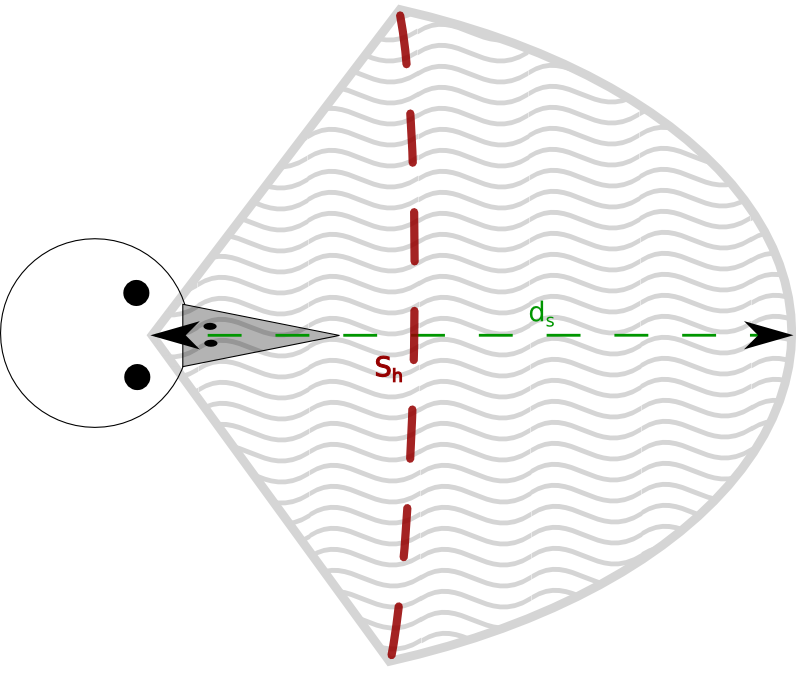
\includegraphics[scale=0.17]{images/hFow}
	\label{fig:hFOV}
	\caption{Birds horizontal field of view. }
\end{figure}
\end{columns}
\end{center}
\end{frame}


\begin{frame}
	\begin{table}[h!]
		\centering
		\begin{tabular}{ |l | l |l| }
			\hline
			\textbf{Name}& \textbf{Symbol} & \textbf{Dimension}\\ \hline
			
			Mass & \(m\) & \(\dimens{L}\) \\
			Peak Velocity & \(v_p\)  & \( \dimens{L} \dimens{T^{-1}}\)  \\
			Thrust 	& \(a\) & \( \dimens{L} \dimens{T^{-2}}\)  \\
			Horizontal Range of View & \(s_h\) & \(-\) \\ 
			Vertical Range of View & \(s_v\) 	& \(-\) \\
			Sight Distance & \(d_s\) & \( \dimens{L}\) \\
			Minimum Distance & \(d_{min}\) & \( \dimens{L}\)\\
			Alignment Radius & \(d_a\) & \( \dimens{L}\)  \\
			Other Species Avoidance Radius & \(r_s\) & \( \dimens{L}\)\\
			Predator Avoidance Radius & \(r_p\) & \( \dimens{L}\) \\
			Maximum Turn & \(\theta_{max}\) & \( rad \dimens{s^{-1}} \)\\
			Wander Distance & \(w_d\) & \( rad \dimens{s^{-1}} \) \\
			Wander Radius & \(w_r\)	& \( rad \dimens{s^{-1}} \) \\ 
			\hline
		\end{tabular}
	\end{table}
\end{frame}



\subsection{Bird's field of view }
\begin{frame}
\textcolor{blue}{\underline{Bird's field of view:}}

Each bird has a limited visual capacity described by its field
of view (FOV, $\mathcal{F}_p$). Let $\vb{p'_n}=\expval{p^x_n-v^x_o,p^y_n-v^y_o,p^z_n-v^z_o}$ the position vector of the object $n$ in the $o$'s frame of reference, then $n$ is $o$'s neighbour if and only if the followings hold:
\begin{equation}
\label{eq:fov1}
	\delta_s = || \vb{p_o} - \vb{p_n} ||,\; \delta_s \leq d_s  \notag 
\end{equation}
 
\begin{equation}
\label{eq:fov2}
	- \; \frac{s_h}{2} \leq \theta \leq \frac{s_h}{2}, \ \ \ \  - \; \frac{s_v}{2} \leq \phi \leq \frac{s_v}{2} \notag
\end{equation}

where $s_h$ is the maximum horizontal range of view, $s_v$ is the maximum vertical range of view and 
\begin{align*}
 &\phi = \arccos
	\left(\frac{p'^z_n}{\sqrt{(p'^x_n)^2 + (p'^y_n)^2 + (p'^z_n)^2}}\right), \ \  
	\theta = atan2 \left(\frac{p'^y_n}{p'^x_n} \right)  \notag
\end{align*}
\end{frame}

\subsection{Cohesion, separation and alignment }
\begin{frame}
\textcolor{blue}{\underline{Cohesion:}}
In formal terms \(\vec{C}_b^i\), the bird $b$'s centroid at time $i$, is given by:
\begin{center}
\begin{columns}
\column{.65\textwidth} 


\begin{align}
 \vec{C}_b^i = \frac{1}{|\mathcal{N}_b|}\sum_{n=1}^{|\mathcal{N}_b|}{\vec{p}_n  \frac{d_{i,j}}{d_s}} \notag
\end{align}

\column{.45\textwidth} 
\begin{figure}[h!]
		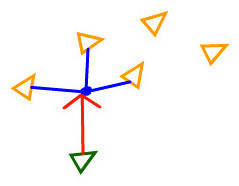
\includegraphics[scale=0.4]{images/cohesion}
		\label{fig:vFOV}
		%\caption{Birds vertical field of view. }
\end{figure}	


\end{columns}
\begin{enumerate}
\item \(\mathcal{N}_b\) the set of birds in b's FOV.
\item \(\vec{p}_n\) is the position of $n \in \mathcal{N}_b$, set of neighbours
\item \(d_{i,j}\) is the distance between bird \emph{b} and its neighbour
	\emph{c}

\end{enumerate}

The $b$'s cohesion vector \(\vec{v}_c\) is then defined as follows.

\begin{equation}
\vec{v}_c^i =
	\begin{cases}
	 \frac{\vec{C}_b^i - \vec{p}_b}{|| \vec{C}_b^i - \vec{p}_b ||} +
		a, &\mbox{ if } 0 < |\vec{v}_d| \leq v_p \\
		v_p, &\mbox{ otherwise }  \notag
	\end{cases}
\end{equation}

\end{center}

\end{frame}

\begin{frame}
\textcolor{blue}{\underline{Separation:}}
A bird try to keep certain distance between itself and
its neighbours. Bird $b$'s separation velocity $\vec{S}_b^i$ at time $i$ is given
by:


\begin{equation}
\vec{S}_b^i = 
	\begin{cases}
	 \left[\sum_{j \in \mathcal{N}_b}{\frac{\vec{p}_b -
\vec{p}_j}{||\vec{p}_b - \vec{p}_j||}} \;f_s\right] + a ,&\mbox{if } 0 < |\vec{S}_i|
\leq v_p\\
		v_p, &\mbox{ otherwise }  \notag
	\end{cases}
\end{equation}

\begin{columns}
\column{.55\textwidth} 

\begin{enumerate}
\item \(\mathcal{N}_b\) is the set of neighbours, %the number of ,
\item $
	f_s = \begin{cases}
	0 &\mbox{ if }  d_{i,j} > d_{min}\\
	1 - \frac{d_{i,j}}{d_{min}} &\mbox{ otherwise} \notag
	\end{cases}$
\end{enumerate}

\column{.35\textwidth} 
\begin{figure}[h!]
		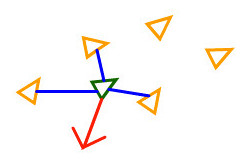
\includegraphics[scale=0.4]{images/separation}
		\label{fig:vFOV}
		%\caption{Birds vertical field of view. }
\end{figure}	


\end{columns}


$d_{min}$ is the minimum distance between two birds to avoid collision.
\end{frame}

\begin{frame}
\textcolor{blue}{\underline{Alignment:}}
Bird $b$'s alignment \(\vec{A}_b^i\) is here defined as %(equation \ref{eq:alignment})

\begin{columns}
\column{.55\textwidth} 
\begin{align}
  \vec{A}_i = \left[\sum_{j \in \mathcal{N}'_b}{\vec{v_j}}\;f_a\right] + a, \;\;0 < |\vec{A}_i| \leq v_p \notag
  \label{eq:alignment}
\end{align}

\column{.35\textwidth} 
\begin{figure}[h!]
		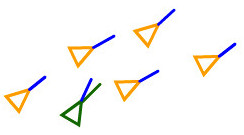
\includegraphics[scale=0.4]{images/alignemtn}
		\label{fig:vFOV}
		%\caption{Birds vertical field of view. }
\end{figure}	


\end{columns}

\begin{enumerate}
\item \(\mathcal{N}'_b \subseteq \mathcal{N}_b\) is the set of birds considered by $b$ for the alignment (e.g. the nearests).
\item \(\vec{v}_j\) is the $j$'s velocity.
\item \(f_a\) is the alignment coefficient. Let \(d_{i,j}\) the distance between bird \emph{i} and \emph{j} then \(f_a\) is given by:

\begin{equation*}
	f_a = \begin{cases}
	0 &\text{, if $ d_{i,j} > d_a$}\\
	1- \frac{d_{i,j}}{d_a} &\text{, otherwise} \notag
	\end{cases}
\end{equation*}
$d_a$: maximum distance bird consider to align 
\end{enumerate}
\end{frame}

\subsection{Other species and predator avoidance}
\begin{frame}
\textcolor{blue}{\underline{Other species and predator avoidance:}}
\textsc{ACIADDRI} is a multi-agent with multiple group model:


 \textbf{1. Other species avoidance}
	
	This behaviour is similar to \textit{separation}  with the difference that a only birds from other species are taken into consideration. In formal terms the other specie avoidance vector  $(\vec{\tau}_i) $is given by:
	
	\begin{equation}
	\vec{\tau}_i = 
		 \left[\sum_{j \in \mathcal{N}_b}{\frac{\vec{p}_b -\vec{p}_j}{||\vec{p}_b - \vec{p}_j||}} \;f_s\right] + a  \notag
	\end{equation}
	where:
	
	\begin{enumerate}
	\item \(\mathcal{N}_b\) is the number of neighbours of specie different from the one of $b$,
	
	\item $
		f_s = \begin{cases}
		0 &\mbox{ if }  d_{i,j} > r_s\\
		1 - \frac{d_{i,j}}{r_s} &\mbox{ otherwise} \notag
		\end{cases}$ \hfill \\
		$ r_s$ is the minimum distance bird avoid other species
	\end{enumerate}
\end{frame}

\begin{frame}
\textbf{2. Predator avoidance}

The predator avoidance vector is computed by taking in consideration position and velocity (speed and heading) of all the  predators within the bird's FOV.
The predator avoidance vector $\vec{\Gamma}_b^i$ is defined as follows:
	
	\begin{align}
	\vec{\Gamma}_b^i = \left[\sum_{j \in \mathcal{P}_b }{\frac{\vec{p}_i -
	(\vec{p}_j+\vec{v}_j)}{||\vec{p}_i - (\vec{p}_j+\vec{v}_j)||}} \;f_{p}\right] +
	a, \;\;0 < |\vec{\Gamma}_i| \leq v_p \notag
	\end{align}
	
	where:
	
	\begin{enumerate}
	\item \(\mathcal{P}_b\) is the $b$'s set of predators
	\item $	f_{p} = \begin{cases}
		0 &\mbox{ if }  d_{i,j} > r_p\\
		1 - \frac{d_{i,j}}{r_p} & \mbox{ otherwise}
		\end{cases}
	$ \hfill \\
	 is the predator avoidance coefficient, where $r_p$ is the  minimum distance bird avoid predator.
	\end{enumerate}
\end{frame}

\begin{frame}
\textcolor{blue}{\underline{Wandering:}}

When the neighbourhood  of a bird is empty it flies pseudo-randomly in the space. This kind of behaviour is called \textit{wandering}. 
Wandering is obtained combining a current and a random direction 
\[
\vec{s} = rand()
\]
\begin{equation}
    \vec{\omega}_b^i =  
		\begin{cases} 
			0 & \mbox{if } \mathcal{N}_b \neq \emptyset \\ 
			\frac{\vec{s}}{|\vec{s}|}\;w_r+w_d,\; 0 < |\vec{\omega}_b^i| \leq v_p &  \mbox{otherwise}  \notag
		\end{cases}
\end{equation}
Where 
\begin{itemize}
\item $w_d$ is the maximum wandering distance;
\item $\vec{w_r}$ is the radius wandering from the target;
\end{itemize}

\end{frame}

\subsection{Flight model}
\begin{frame}
\textcolor{blue}{\underline{Flight model:}}

Bird $b$ flight at step $i$ is described by 
\begin{equation}
\vec{ p_b}^i = < p_x^i , p_y^i , p_z^i >, \ \ \ \ \vec{v_b}^i = < v_x^i , v_y^i , v_z^i > \notag
\end{equation}
The evolution of the bird's velocity over time is regulated
by 
\begin{equation}
\vec{v}_b^{i+1} = (r sin\theta' cos \phi', \ r sin\theta' sin \phi', \ r cos \theta') \notag
\end{equation}
where:
\begin{itemize}
  \item $
     \theta' = \begin{cases}
    \theta_d &\mbox{ if }  |\theta_b - \theta_d| < \theta_{max}\\
    \theta_b + \theta_{max} &\mbox{ otherwise }\\
    \end{cases}
  $ \hfill \\
  \medskip
    \item $
     \phi' = \begin{cases}
    \phi_d &\mbox{ if }  |\phi_b - \phi_d| < \phi_{max}\\
     \\
    \phi_b + \phi_{max} &\mbox{otherwise}\\
    \end{cases}
  $ \hfill \\ 
\end{itemize}
\end{frame}
   
\begin{frame}
The polar angle $\theta_d$ and the azimuth angle $\phi_d$ are associated to 
\begin{equation}
 \vec{v}_d^i = \mu_c \vec{v}_c + \mu_s\vec{v}_s + \mu_a \vec{v}_a + \mu_{A} (
\vec{{\tau}_i} + \vec{\Gamma}_i ) + \vec{\omega}_i \notag
\end{equation}
 where

\begin{itemize}
	\item $\mu_c$, $\mu_s$, $\mu_a$ are the cohesion, separation and alignment coefficient (social coefficients) and $\mu_A$ is the avoidance coefficient,

\item  $\vec{v}^i_c$,$\vec{v}^i_s$, $\vec{v}^i_a$ are the  \textit{social velocities}: 
    \begin{itemize}
    \item $\vec{v}^i_c$, the cohesion velocity,
    \item $\vec{v}^i_s$, the separation velocity, 
    \item  $\vec{v}^i_c$, the align velocity.

    \end{itemize}
    
\item  $\theta_d,\theta_b$ are the polar angle of the velocity vector
  $\vec{v}^i_b$ and $\vec{v}^i_d$ respectively.
\item $\phi_d,\phi_b$ are the azimuthal angle of the velocity vector
  $\vec{v}^i_b$ and $\vec{v}^i_d$ respectively.
  \item $\vec{\omega}_i$ is the wondering vector.
\end{itemize}
\end{frame}


\section{GPGPU parallel implementation and results}
\begin{frame}{GPGPU parallel implementation }
In this work we adopt GPUs and the CUDA framework to
accelerate the flocking simulation of a large number of boids
using the model presented  in an environment
with a number of agents up to $5x10^6$. 
We produced two different parallel
versions adopting the typical host-managed accelerated
program structure:
\begin{itemize}
	\item Initialization of data structures on \emph{CPU}
	\item Data transfer from \textbf{\emph{CPU} to \emph{GPU}}
	\item Kernels execution on \emph{GPU}
	\item Copying the result back from \textbf{\emph{GPU} to \emph{CPU}}
\end{itemize}
The parallelization strategy is designed with the purpose to avoid as much
as possible the very undesirable data copy from \emph{host to device}, or vice versa.

\end{frame}

\begin{frame}
\begin{itemize}
\item The computation of $\vec{p}_b^{i+1}$ 
and $\vec{v}_b^{i+1}$  is entirely performed on GPU
and implemented as composition of CUDA kernels.
\item Parameters are stored in constant memory for fast access.
\item An OpenGL 3D visualization tool comes with the simulation
system and permits real time and interactive rendering of the
flocking model.
\end{itemize}
\end{frame}

\subsection{Na\"{i}ve version}
\begin{frame}
\textcolor{blue}{\underline{Na\"{i}ve version:}}

Each agent is mapped to a CUDA thread organized in a 1D block-grid structure. 
\begin{itemize}
\item All data resides in global memory and user managed cache (shared memory) is
unused.
\item This version already gives rise to a
speedup of $ \thickapprox 20x$.
\item An optimization was carried out by considering the \textit{If-Divergence mitigation}
\item The serialization presents a performance loss. 
\end{itemize}
\end{frame}
\subsection{Shared memory version}
\begin{frame}
\textcolor{blue}{\underline{Shared memory version:}}

% XXX vuoi aggiungere una slide sulla shared memory (imagine tipica) ??
The shared memory is exploited in order to cache
bird's frequently accessed data.
\begin{itemize}
\item Shared memory is much faster than global memory,
\item although it is of limited capacity (and
depends on compute capability of the device), only accessible at block level and cleared at
each kernel invocation.
\item The adopted strategy divides the computation in a number
of phases that depend on the chosen block size. Each phase
can be then performed exploiting the fast memory.
\end{itemize} 
Different tests were carried out  by considering
different number of boids and an environment composed of
$1000 \times 1000 \times 1000$ cells. Each simulation was carried out for
$10^4$ time steps.
\end{frame}
\begin{frame}
Three devices were adopted for testing different CUDA
version of the model: the high-end GTX 980 and a GT 635M a low-end mobile chip.

The followings are shown the execution times (in seconds) of the na$\ddot{i}$ve and shared memory version:

\begin{table} [h!]
	\centering
		\begin{tabular}{|l |l |l| l|}
	\hline
	\# birds & Sequential & GT	635M ($\times$) & GTX 980 ($\times$) 
	\\
	\hline
	
	1024  	& \(263.9\) 	& $29.1$, ($9,07$) 	& $10.5$, ($25,13$) \\
	5120  	& \(4913.0\) 	& $574.4$, ($8,55$) 	& $51.7$, ($95,02$)  \\
	10240 	&  $19074.5$ 	& $2241.6$, ($8.51$) 	& $109.0$, ($174,99$)  \\
	15360 	& \(43332.3\) 	& $5004.7$, ($8.65$) 	& $235.2$, ($184,23$)  \\
	20480  	& 86065.7 		& $8868.9$, ($9,70$) 	& $312.5$, ($275.408$) \\
	40960  	& 452423.1 		& - 						& $1023.8$, ($441.90$)  \\
	81920  	& 1966134.9 	& - 						& $3663.5$, ($536,70$)  \\
	163840  & 8003173.0 	& - 						& $14877.4$, ($537,94$)	 \\
	327680  & 35815012.0 	& - 						& $58003.0$, ($617,47$)  \\
	\hline
	\end{tabular}
	\caption{Timings for the Parallel CUDA Na\"ive implementation}. Number in brackets represent speedups.
	\label{tab:naive}
\end{table}
\end{frame}

%XXX metterei anche un grafico per i speedup, per evidienzare gli ottimi risultati

\begin{frame}
Timing (in seconds) for the Parallel CUDA shared memory implementation:
\begin{table} [h!]
	\centering
	\begin{tabular}{|l |l |l| l|}
	\hline
	\# birds & Sequential & GT	635M & GTX 980
	\\
	\hline
	

	1024  & \(263.9\) & $19.9$ & $7.9$  \\
	5120  & \(4913.0\) & $366.3$ & $34.6$  \\
	10240 &  $19074.5$ & 1398.7 & 96.5  \\
	15360  & \(43332.3\) & $3110.0$ & $154.9$  \\
	20480  & 86065.7 & 5522.0 & $280.8$ \\
	40960  & 452423.1 & - & $825.4$ \\
	81920  & 1966134.9 & - & $3307.2$ \\
	163840  & 8003173.0 & - & $13565.9$ \\
	327680  & 35815012.0 & - & $54113.4$  \\
	\hline
	\end{tabular}
	%\caption{Timing (in seconds) for the Parallel CUDA shared memory implementation}
	\label{tab:ifdiv}
\end{table}
We see an evident cut down of computational time by GPGPU use.
\end{frame}
\section{Conclusions}
\begin{frame}
\begin{itemize}
\item Starting from Reynolds's behavioural model, we have 
presented a preliminary multi-agent and multiple group approach for bird flocking coupled with an efficient implementation by means of the CUDA framework.
\item We have proven the full suitability of the GPGPU paradigm for efficiently simulating multi-agent systems.
\item Future developments:
\begin{itemize}
\item improve the bird's light modelling to better adhere with aerodynamics theory;
\item adding the possibility of the environment to contain obstacles, and the usage of multi-gpu hardware.
\end{itemize}
\end{itemize}
\end{frame}

\begin{frame}
\begin{center}
\begin{huge}Thanks for your kind attention! \end{huge}
\end{center}

\end{frame}
\end{document}